\chapter{Modelado del problema}\label{formulacion}

El ``jopara'', escrito y hablado en Paraguay, seg\'un Lustig (1996) ``en sentido estricto escapa a la condici\'on de una \textit{lengua}'' y es mejor descrito como una ``\textit{mezcla de lenguas} que como una \textit{lengua mezclada}''. Compuesto por el uso de palabras tanto del espa\~nol como del guaran\'i en una misma entidad de texto (documento, oraci\'on o incluso palabra), no se trata de un lenguaje oficial, ni tampoco de un dialecto por lo que no se disponen de reglas ni regulaciones formales expl\'icitas para la construcci\'on de oraciones. Este hecho representa la dificultad principal para la creaci\'on de un l\'exico as\'i como para el entrenamiento de un clasificador.
\newline

En el lenguaje natural utilizado entre las personas para comunicarse, se puede notar el uso frecuente del jopara, incluso en las redes sociales. Esto nos lleva considerar relevante su uso para el an\'alisis de sentimientos, particularmente porque las palabras originadas del guaran\'i son generalmente utilizadas para enfatizar sentimiento. Por ejemplo, en la oraci\'on \textit{``Kore! Ndoikoi ko aparato, encima que lo compr\'e reci\'en''}, las palabras ``kore'', ``ndoikoi'' y ``ko'' est\'an escritas en guaran\'i, y el resto de ellas en espa\~nol. Claramente, en esta oraci\'on, el indicador m\'as evidente de negatividad en esta oraci\'on es la interjecci\'on que la inicia.
\newline

En este cap\'itulo, presentamos el modelado propuesto para aplicar las t\'ecnicas de categorizaci\'on descriptas en el cap\'itulo anterior sobre el lenguaje abordado. Describimos algunos patrones de formaci\'on de palabras en el jopara, el formato de entrada de los textos en Twitter y establecemos algunas reglas de preprocesamiento para lograr una selecci\'on adecuada de atributos de entrada para los clasificadores.
\newline \newline

\section{Caso de estudio: Reacciones de clientes de una compa\~n\'ia de telecomunicaciones}

Con el fin de efectuar un an\'alisis que permita detectar la polaridad de los sentimientos en un escenario dado, tomamos en cuenta las opiniones expresadas por los usuarios de una compa\~n\'ia de telecomunicaciones que domina gran parte de dicho mercado, en un mediador de redes sociales de uso masivo. Twitter es una de las herramientas de interacci\'on m\'as populares entre los usuarios de Internet, y dado su formato libre y corto de mensajes adem\'as de su accesibilidad, recopilamos un corpus de 20.000 textos que representan interacciones de los usuarios con la compa\~n\'ia en cuesti\'on, es decir los mensajes que contengan una menci\'on de la cuenta de dicha compa\~n\'ia en la red de Twitter.
\newline

Presentamos entonces, el an\'alisis sobre un corpus compuesto por una variedad de lenguajes. Si observamos los contenidos compartidos por los usuarios en el corpus extra\'ido, notamos que las oraciones est\'an escritas no solamente en los lenguajes nativos oficiales de Paraguay sino que adem\'as en jopara, ingl\'es y portugu\'es. Por tanto, proponemos el tratamiento de dichos lenguajes en conjunto mediante la aplicaci\'on de los m\'etodos existentes de an\'alisis, centr\'andonos principalmente en la selecci\'on de atributos y la calibraci\'on de los par\'ametros de entrada para los algoritmos.
\newline

Previamente a la descripci\'on general del procedimiento seguido, describimos las caracter\'isticas del formato de los mensajes compartidos en Twitter (tuits).

\section{Caracterizaci\'on de mensajes en Twitter}

Los mensajes compartidos en Twitter poseen varias caracter\'isticas \'unicas, que los diferencian de los dem\'as corpus de datos citados previamente. (Go y otros, 2009) identifican cuatro de ellas:

\begin{itemize}
\item \textbf{Longitud m\'axima:} Cada publicaci\'on puede estar compuesta por una cantidad m\'axima de 140 caracteres, incluyendo signos de puntuaci\'on y s\'imbolos.
\item \textbf{Alta disponibilidad:} La API de Twitter permite obtener tuits libremente, a trav\'es de su funci\'on de b\'usqueda. Mediante esta funci\'on es posible recolectar una cantidad de tuits considerable para conformar los conjuntos de entrenamiento y de evaluaci\'on.
\item \textbf{Modelo del lenguaje:} Los mensajes de Twitter pueden ser generados desde diversos dispositivos, incluyendo los tel\'efonos celulares. Esto lleva a que los errores ortogr\'aficos y expresiones informales se hagan mucho m\'as frecuentes en comparaci\'on a otros dominios.
\item \textbf{Dominio:} Los tuits se refieren a diversos temas, lo cual es relevante puesto que un gran porcentaje de estudios pasados fueron centrados en un dominio espec\'ifico.
\end{itemize}

Existen adem\'as ciertas convenciones de lenguaje de los tuits:
\begin{itemize}
\item ``RT'' es un acr\'onimo de retuit, que se coloca delante de un mensaje para indicar que el mismo est\'a siendo repetido o compartido.
\item El caracter ``\#'' es utilizado para marcar, organizar y clasificar tuits por temas o categor\'ias.
\item El caracter ``@'' es empleado para referirse a una cuenta por su nombre de usuario.
\end{itemize}

Es frecuente adem\'as que los tuits vayan acompa\~nados de emoticones y v\'inculos de Web. La influencia de las caracter\'isticas de estos mensajes en nuestra propuesta es abordada en la siguiente secci\'on.

\section{Procedimiento general}\label{procedimiento}
El procedimiento seguido para generar los resultados desde los tuits recolectados inicialmente se muestra en la Figura \ref{overview}. Como se puede observar, en algunas etapas del mismo se producen ciertos productos intermedios significativos como el corpus, el l\'exico y el conjunto de entrenamiento antes de llegar a los resultados.
\newline

\begin{figure}[h]
\centering
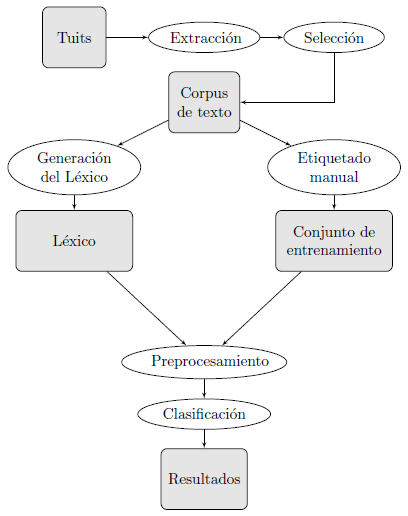
\includegraphics[width=0.7\textwidth]{overview.png}
\caption{Vista general del proceso seguido para obtener los resultados.}
\label{overview}
\end{figure}

Las etapas de las que se compone el proceso son las siguientes:
\begin{itemize}
\item \textbf{Extracci\'on:} Recolectamos inicialmente 20.000 tuits con alguna menci\'on a la compa\~n\'ia objeto. Esto fue logrado mediante el uso de la API de Twitter \footnote{https://dev.twitter.com/docs/api (Version 1.1)}.  Cada tuit retornado en una consulta contiene varios atributos relativos a las interacciones entre usuarios, de los cuales utilizamos \'unicamente el cuerpo de texto, como objeto de estudio, y el n\'umero identificador de cada uno, para evitar duplicaciones; en tanto, los dem\'as atributos son irrelevantes para los objetivos trazados en este trabajo. Para obtener la cantidad final de tuits, varias consultas debieron ser ejecutadas debido a que existe un l\'imite de 450 mensajes recuperables por cada consulta en la versi\'on utilizada de la herramienta. El per\'iodo de extracci\'on estuvo comprendido entre Marzo y Junio del 2013.
\item \textbf{Selecci\'on:} Para limitar el trabajo manual realizado en el proceso, aleatoriamente seleccionamos (con un muestreo equiprobable) unos 3.000 tuits que componen el corpus de texto. De esta cantidad seleccionada, el total de tuits fue utilizado para construir el l\'exico, mientras que 1.500 de ellos fueron etiquetados manualmente para entrenar los clasificadores. Adem\'as, un grupo independiente de 300 tuits fue seleccionado para conformar un conjunto independiente de evaluaci\'on.
\newline \newline
La etapa de selecci\'on implica algunas operaciones de limpieza para tratar los retuits  (ver secci\'on anterior) en dos casos posibles. El primer caso trata de los retuits de alg\'un mensaje compartido por un usuario, que resultan despreciables para este an\'alisis pues buscamos heterogeneidad en los conjuntos de entrenamiento. Por el otro lado, los retuits de los mensajes escritos por la propia cuenta de la compa\~n\'ia, que no resultan relevantes puesto que el objetivo consiste en describir las reacciones de sus clientes. En estos casos, fueron seleccionados aleatoriamente nuevos tuits de reemplazo para mantener el tama\~no de los conjuntos especificados en el p\'arrafo anterior.
\item \textbf{Generaci\'on del l\'exico y etiquetado manual:} \'Estos son los procedimientos que implican la mayor porci\'on del trabajo manual durante el proceso. El l\'exico generado contiene una lista de unigramas etiquetados seg\'un el lenguaje de origen, clasificaci\'on gramatical y frecuencia en el corpus con fines estad\'isticos. Adem\'as, unas listas de palabras orientadas tanto positiva como negativamente y una de \textit{stopwords} fueron elaboradas para ser utilizadas en la categorizaci\'on. Los detalles de construcci\'on de dichas listas se describen en la siguiente secci\'on.
\newline \newline
El etiquetado manual de los tuits es efectuado con el fin de generar los conjuntos de entrenamiento para los clasificadores de m\'aquina. Fueron definidas tres clases, por polaridad de sentimientos: positivas, negativas y neutrales. Como el caso de estudio presentado es orientado a un dominio espec\'ifico, varios de los textos fueron clasificados de acuerdo a la sensaci\'on percibida relativa al dominio en cuesti\'on. Por ejemplo, algunos tuits positivos son respuestas a algunos anuncios comerciales o reacciones a precios divulgados por la compa\~n\'ia; los negativos son quejas referentes a los productos o a ciertos servicios prestados; en tanto, los neutrales son simples preguntas o comentarios relativos a eventos patrocinados por la compa\~n\'ia. Algunos ejemplos de tuits etiquetados pueden verse en el Cuadro \ref{etiquetado}, en los cuales la menci\'on a la compa\~n\'ia est\'a representada por la palabra \textit{``@telecom''}.

\begin{table}[htb] 
\centering
\begin{tabular}{|p{10cm}|p{2cm}|}
\hline
\textbf{Tuit}	&	\textbf{Polaridad}	\\
\hline
``Excelente el servicio online @telecom''	&	Positiva	\\
\hline
``Buen servicio de Internet @telecom al tener un problema con el aparato enseguida vinieron a cambiarnos!''	& Positiva	\\
\hline
``Ahora ya ni hablar tranquilo se puede de @telecom te cortan!!!''	&	Negativa	\\
\hline
``Que peor serviciooooo!!! Grrrr!! @telecom''	&	Negativa	\\
\hline
``C\'omo hago para bloquear un n\'umero? @telecom''	&	Neutral	\\
\hline
``Hola, el Nokia Lumia 820 tienen? @telecom''	&	Neutral	\\
\hline
\end{tabular}
\caption{Etiquetado de tuits por polaridad}
\label{etiquetado}
\end{table}

\item \textbf{Preprocesamiento:} Algunas reglas de preprocesamiento fueron establecidas con el fin de mejorar la selecci\'on de atributos y consecuentemente, la calidad de los resultados obtenidos. Tales reglas permiten adem\'as que los atributos del conjunto de entrenamiento describan mejor la polaridad de un texto compuesto por alguna combinaci\'on de ellos. Las reglas son las siguientes:
\begin{enumerate}
\item Los \textit{links} (v\'inculos de Internet) son eliminados debido a que no conllevan carga alguna de polaridad respecto a una entidad objeto.
\item Las ocurrencias seguidas de un mismo caracter son reemplazadas por una ocurrencia singular del mismo caracter, para tratar el fen\'omeno conocido como ``prolongaci\'on de palabras'', exceptuando los d\'igrafos propios del espa\~nol como ``ll'' y ``rr''. Algunos ejemplos pueden verse en el Cuadro \ref{lengthening} De esta manera, logramos que las mismas palabras sean reconocidas como un atributo en com\'un si existen varias ocurrencias de ellas, puesto que los \textit{tokens} deben ser id\'enticos para el efecto. En el trabajo de Brody y Diakopoulos (2011) se trata m\'as minuciosamente este fen\'omeno.
\newline

\begin{table}[htb] 
\centering
\begin{tabular}{|p{5cm}|p{5cm}|}
\hline
\textbf{Forma extendida}	&	\textbf{Forma normalizada}	\\
\hline
servicioooooo				&	servicio	\\
\hline
decodificador??????????		&	decodificador?	\\
\hline
Grrrrr						&	Grr	\\
\hline
\end{tabular}
\caption{Normalizaci\'on de palabras extendidas}
\label{lengthening}
\end{table}

\item Las entidades particulares del lenguaje HTML y los caracteres del formato de codificaci\'on UTF son reemplazados por los s\'imbolos equivalentes. Por ejemplo, ``\&lt'' es reemplazado por ``$<$'', ``\&gt'' por ``$>$'', entre otros s\'imbolos.



\item Los emoticones son clasificados manualmente entre positivos y negativos, de tal manera que al final existen solamente dos atributos gen\'ericos para los emoticones,  uno para cada carga de polaridad respectivamente. Dichas representaciones gen\'ericas sirven de contrapeso para los \textit{tokens} de emoticones sarc\'asticos en los clasificadores de m\'aquina.
\item Los \textit{tokens} que representan menciones de cualquier usuario son removidos puesto que no conllevan carga alguna de polaridad.
\item Las palabras que llevan acento son reemplazadas por su equivalente sin acentos. Esto es debido a que tanto en espa\~nol como en guaran\'i existen dos tipos posibles de acentos, los cuales son `` \'\ ''  y `` \^\ '' . Dado que es frecuente observar errores de escritura de los usuarios en lenguaje natural como por ejemplo, palabras sin acentos, tildes ubicadas incorrectamente o diferentes representaciones de ellos debido a las diversas configuraciones de teclas, este reemplazo es efectuado con el fin de unificar atributos en caso de ocurrencias iguales. Teniendo en cuenta esta regla, identificamos cuatro casos posibles, que son los siguientes si los colocamos a modo de ejemplo sobre la vocal ``a'': ``\'a'', ``\`a'', ``\^a'', ``\"a''. 
\item Algunos caracteres o s\'imbolos frecuentes (diferentes de las letras del abecedario) son removidos. Esto tambi\'en es llevado a cabo con la finalidad de unificaci\'on de atributos. Existen casos de puntuaci\'on como el punto, la coma, los par\'entesis y otros que formar\'ian parte de un \textit{token} si no fuesen removidos. Adem\'as, como fue descripto en la secci\'on anterior, existe la convenci\'on del caracter ``\#'' en Twitter, el cual es removido del inicio de las palabras. La lista completa de caracteres eliminados se detalla en el Cuadro \ref{caracteres}.
\newline

\begin{table}[htb] 
\centering

$
\begin{array}{|c|c|c|c|c|c|c|c|c|c|c|c|}
      \hline
      \#	&	@	&	*	&	(	&	)	&	$?`$	&	
      ?		&$	!` $&	!	& 	\lbrace	&	\rbrace	&	/ \\
      \hline
      .		&	,	& \backslash	&	:	& -	& \_ & = & \% & + & ; & < & >  \\
      \hline
\end{array}
$
\caption{Caracteres eliminados en el preprocesamiento}
\label{caracteres}
\end{table}

\item Algunos bigramas considerados neutrales son eliminados, pues consideramos que no representan impacto alguno referente a polaridad en las opiniones, incluso en las neutrales. Estas son las expresiones de saludos tales como ``buenos d\'ias'' y otras similares; son utilizadas de manera respetuosa precediendo a alguna pregunta, comentario, sugerencia o incluso una queja.
\end{enumerate} 
\item \textbf{Categorizaci\'on:} Esta etapa consiste en la aplicaci\'on de los algoritmos antes descriptos para estimar a cu\'al de las clases pertenece cada entrada. Mayores detalles sobre la configuraci\'on de cada algoritmo son descriptos en las siguientes secciones.
\end{itemize}

Presentado el procedimiento general, centramos las siguientes subsecciones en el abordaje de las tareas de configuraci\'on y, en algunos casos codificaci\'on, de los clasificadores basados tanto en l\'exico como en aprendizaje de m\'aquina.

\section{Desarrollo del l\'exico}

Las estrategias basadas en l\'exico son tambi\'en ampliamente utilizadas para la categorizaci\'on de sentimientos. Para aplicar las t\'ecnicas basadas en este enfoque, fue necesario desarrollar un l\'exico desde el principio, debido a que no existen a\'in listas de palabras disponibles para este tipo de lenguaje.
\newline 

Como fue descrito antes, la cantidad de tuits seleccionados para la construcci\'on del l\'exico fue de 3.000. El primer paso consisti\'o en obtener una lista de todas las palabras presentes en el corpus con su frecuencia total y su frecuencia de aparici\'on en diferentes tuits, respectivamente. Este paso fue realizado mediante la utilizaci\'on de la librer\'ia Lucene \footnote{https://lucene.apache.org/} de Apache.
\newline 

Con dicha lista disponible, el trabajo manual debi\'o ser realizado. Una de las tareas consisti\'o en determinar la categor\'ia ling\"u\'istica y la categor\'ia l\'exica de cada palabra. Adem\'as, fue desarrollada una lista de palabras con polaridad orientada positivamente y otra lista con aquellas que tienen orientaci\'on negativa.

\subsection{Categorizaci\'on ling\"u\'istica y l\'exica}\label{sec:categorizacion}

Las categor\'ias fueron definidas con el fin de determinar la distribuci\'on de las palabras y su influencia en el corpus. Seis categor\'ias ling\"u\'isticas fueron identificadas en el texto: Espa\~nol, Guaran\'i, Jopara, Ingl\'es, Portugu\'es y Emoticones. Las categor\'ias Guaran\'i y Jopara existen separadamente debido a que algunas palabras son genuinas del idioma (podemos encontrarlas en un diccionario de guaran\'i) mientras que otras son palabras del espa\~nol con prefijos o sufijos del guaran\'i. Por ejemplo, en la expresi\'on ``ndaigustoi'' \textit{(no es divertido)} el lema es ``gusto'', una palabra del espa\~nol, mientras que el prefijo ``ndai'' y el sufijo ``i'' indican negaci\'on y provienen del guaran\'i. Entonces, a estas palabras no podemos considerarlas como propias del espa\~nol ni tampoco del guaran\'i, entonces las clasificamos como pertenecientes a la clase Jopara. Existen adem\'as expresiones que presentan el caso inverso, es decir una palabra cuyo lema pertenece al guaran\'i y el sufijo y/o prefijo al espa\~nol, las cuales tambi\'en pertenecen a la misma categor\'ia. Las clases Ingl\'es y Portugu\'es fueron definidas debido a que fueron identificadas palabras provenientes de dichas lenguas durante la generaci\'en del l\'exico. Los resultados de esta categorizaci\'on se muestran en el Cuadro \ref{cat_ling}.
\newline

Por otro lado, las categor\'ias l\'exicas definidas son: Adjetivos, Adverbios, Art\'iculos, Interjecciones, Sustantivos, Verbos y Emoticones. En este trabajo no efectuamos etiquetado gramatical \textit{(POS tagging)} ni asignamos ponderaciones pero como se puede observar,  algunas categor\'ias conllevan mayor carga de polaridad que otras, por lo que propusimos relacionarlas con las categor\'ias ling\"u\'isticas para medir su influencia en el corpus. El resumen de esta categorizaci\'on es desplegado en el Cuadro \ref{cat_lex}.
\newline

\begin{table}[htb] 
\centering

$
\begin{array}{|c|c|}
      \hline
      \mathbf{Clase}  	& \mathbf{Palabras}	\\
      \hline
      Espa\tilde{n}ol 	& 3802				\\
      \hline
      Guaran\acute{i} 	& 70 				\\
      \hline
      Jopara			& 10				\\
      \hline
      Ingl\acute{e}s	& 72				\\
      \hline
      Portugu\acute{e}s	& 4					\\
      \hline
      Emoticones		& 24				\\
      \hline
\end{array}
$
\caption{Categorizaci\'on ling\"u\'istica del corpus de texto}
\label{cat_ling}
\end{table}

\begin{table}[htb] 
\centering

$
\begin{array}{|c|c|}
      \hline
      \mathbf{Clase}  	& \mathbf{Palabras}	\\
      \hline
      Adjetivos 		& 589				\\
      \hline
      Adverbios 		& 268 				\\
      \hline
      Art\acute{i}culos	& 90				\\
      \hline
      Interjecciones	& 64				\\
      \hline
      Sustantivos		& 1063				\\
      \hline
      Verbos 			& 1888				\\
      \hline
      Emoticones		& 24				\\
      \hline
\end{array}
$
\caption{Categorizaci\'on l\'exica del corpus de texto}
\label{cat_lex}
\end{table}

Considerando nuestro caso particular de estudio, si cruzamos ambas categorizaciones, observamos que las palabras del Guaran\'i y del Jopara est\'an distribuidas en las categor\'ias l\'exicas de la siguiente manera: 20\% son adjetivos, 16,25\%  son adverbios, 17,5\% son interjecciones, 27,5\% son verbos, 7,5\% son sustantivos y 11,25\% son art\'iculos. Como los sustantivos y los art\'iculos son el tipo de palabras que generalmente no conllevan carga de polaridad, podemos observar que la mayor\'ia de las ocurrencias en dichas categor\'ias ling\"u\'isticas son indicadoras de sentimiento.

\subsection{Categorizaci\'on por orientaci\'on de polaridad}

Con el prop\'osito de ejecutar un algoritmo de conteo simple, una categorizaci\'on manual por orientaci\'on de polaridad tambi\'en fue efectuada. La estrategia es simple, pues consiste sencillamente en contar la cantidad de palabras orientadas positivamente y la cantidad de orientadas negativamente por cada instancia, para clasificarla dentro de alguna de las clases. Una entrada es positiva si est\'a compuesta por m\'as palabras de la lista de positivas que por palabras de la lista de negativas; es negativa en caso contrario; mientras que si ambas cantidades son iguales, es clasificada como neutral. De esta manera, no existe una lista de palabras con ``orientaci\'on neutral'', mas una instancia puede pertenecer a dicha clase si hay equilibrio entre palabras orientadas positiva y negativamente. La lista final de palabras positivas contiene 180 entradas mientras que la negativa contiene 634, ambas con su respectiva representaci\'on gen\'erica de emoticones, que cuenta como una \'unica entrada para cada lista. En el Algoritmo \ref{alg:simplecount} se describe la clasificaci\'on de un tuit utilizando las listas generadas. Es importante observar que las palabras que no se encuentran en ninguna de las listas confeccionadas no influyen en el conteo de ocurrencias positivas ni negativas.

\begin{algorithm}
\begin{algorithmic}
\REQUIRE Tuit preprocesado
\ENSURE Polaridad estimada del tuit (positiva, negativa o neutra)
\STATE $cantidadPos = cantidadNeg = 0$ 
\FORALL{$palabra\,$ en $\,tuit$}
\IF{$listaPalabrasPositivas$ contiene a $palabra$}
\STATE $cantidadPos = cantidadPos + 1$
\ELSIF{$listaPalabrasNegativas$ contiene a $palabra$}
\STATE $cantidadNeg = cantidadNeg + 1$
\ENDIF
\ENDFOR
\IF{$cantidadPos > cantidadNeg$}
\STATE $polaridad$ = ``Positiva''
\ELSIF{$cantidadNeg > cantidadPos$}
\STATE $polaridad$ = ``Negativa''
\ELSE
\STATE $polaridad$ = ``Neutral''
\ENDIF
\RETURN $polaridad$
\end{algorithmic}
\caption{Clasificaci\'on de un tuit mediante Conteo Simple seg\'un el L\'exico por polaridad.}
\label{alg:simplecount}
\end{algorithm}

\section{Clasificadores por aprendizaje de m\'aquina}

La tarea de clasificaci\'on por aprendizaje de m\'aquina implica la elaboraci\'on de un conjunto de entrenamiento, la selecci\'on de los atributos y la calibraci\'on de los par\'ametros de entrada que sean requeridos por los algoritmos. En esta secci\'on, describimos estos aspectos de la clasificaci\'on. Las implementaciones utilizadas est\'an incluidas en la colecci\'on de algoritmos de miner\'ia de Weka \footnote{http://www.cs.waikato.ac.nz/ml/weka/}, por lo que describiremos brevemente las particularidades de las funciones utilizadas.
\newline

Los clasificadores de Weka reciben inicialmente un conjunto de entrenamiento. Para ello, deben ser definidos cu\'ales ser\'an los atributos y las instancias del modelo clasificador. Entonces, enfocamos el tratamiento de textos de tal manera que cada palabra diferente encontrada en el conjunto de entrenamiento representa un atributo, mientras que cada tuit representa una instancia del conjunto. Para el efecto, configuramos en Weka un filtro que convierte una oraci\'on dada en un vector de palabras. Adem\'as, debe ser creado un atributo de salida, que formar\'a parte de cada una de las instancias; para el problema tratado, dicho atributo es la orientaci\'on de polaridad, es decir, las etiquetas asignadas manualmente y cuyos valores posibles son Positivo, Negativo o Neutro.
\newline

En la siguientes subsecciones, detallamos las variantes que ofrece cada implementaci\'on respecto a las definiciones de los algoritmos, establecidas en el cap\'itulo anterior, adem\'as de los par\'ametros de entrada que requiere cada una de ellas.

\subsection{Weka - NaiveBayes}

Es un clasificador por el teorema de Bayes que realiza estimaciones de precisi\'on a trav\'es de valores num\'ericos, basado en el an\'alisis de los datos de entrenamiento. Los atributos num\'ericos son utilizados para efectuar un conteo de la cantidad de ocurrencias de cada palabra, en este contexto.  Esta implementaci\'on se vale de una funci\'on heur\'istica para establecer un valor m\'inimo de desviaci\'on est\'andar para los atributos num\'ericos, con el fin de evitar problemas de computaci\'on de los mismos. Esto se debe a que las estimaciones de pertenencia a cada clase son calculadas a trav\'es de la multiplicaci\'on de los valores probabil\'isticos de cada atributo y ello implica operar con n\'umeros muy peque\~nos en ocasiones. Esta funci\'on no requiere de par\'ametros de entrada de mayor relevancia.
\newline

Es importante resaltar que existen adem\'as otras implementaciones del algoritmo de Bayes en Weka, algunas de las cuales son \textit{NaiveBayesUpdateable}, la cual incluye la funci\'on de autoentrenamiento o \textit{NaiveBayesSimple} que no emplea la funci\'on heur\'istica mencionada previamente. El objetivo de este trabajo es realizar la evaluaci\'on con la implementaci\'on sencilla del algoritmo, sin funciones agregadas por lo que no utilizamos el autoentrenamiento; mientras que con la funci\'on simple prove\'ida por Weka, existe el inconveniente de que ella no logra evaluar la totalidad de atributos debido a que algunos de ellos no cuentan con ocurrencia alguna para una de las clases posibles del modelo. Es decir, alg\'un atributo se encuentra definido en el conjunto de entrenamiento por una ocurrencia presentada en alguna de las clases, pero no presentada en las dem\'as, causa posteriormente el problema de que al ser multiplicado, como su valor de probabilidad es cero, resulta tambi\'en en una desviaci\'on est\'andar cero en la estimaci\'on de probabilidades.
\newline

Dado el escenario descripto, efectuamos la clasificaci\'on mediante la funci\'on \textit{NaiveBayes} de Weka; pero adem\'as generamos una implementaci\'on propia del algoritmo en su forma m\'as sencilla, sin funciones heur\'isticas, la cual abordamos a continuaci\'on. 

\subsection{Bayes Ingenuo Simple}

Esta implementaci\'on consiste sencillamente en la aplicaci\'on de f\'ormulas de c\'alculo de probabilidades atributo por atributo para efectuar luego la estimaci\'on de pertenencia de cada instancia a alguna de las clases. La variante introducida se trata de la utilizaci\'on del suavizado de Laplace para resolver el problema de las instancias sin ocurrencias para alguna de las clases. Es decir, evitamos las probabilidades cero en los unigramas no vistos en el c\'alculo de $score$ (definido en la Secci\'on \ref{bayes_sec}).
\newline

El suavizado de Laplace consiste en la introducci\'on de un valor de aproximaci\'on distinto de cero como la cantidad de ocurrencias para un unigrama no visto en el entrenamiento. El primer valor de aproximaci\'on introducido fue 1, es decir una ocurrencia singular ficticia de la instancia; pero esto genera el inconveniente de que, debido al tama\~no peque\~no del conjunto de entrenamiento, dicho valor ficticio aumenta muy considerablemente la masa total de probabilidad del atributo, influyendo fuertemente en los resultados. Luego, dicho valor de aproximaci\'on fue modificado a un n\'umero no entero (0,1), de tal manera que seguiremos evitando el cero en el c\'alculo de $score$, sin permitir a la vez que dicho valor influya fuertemente en las estimaciones.
\newline

El Algoritmo \ref{alg:simplebayes} describe la clasificaci\'on de un tuit preprocesado mediante esta implementaci\'on, en el cual $cantidadOcurrencias$ retorna la cantidad de ocurrencias de una palabra para la clase solicitada (con el suavizado de Laplace si fuese necesario) mientras que $totalPos$ almacena la cantidad total de palabras de cada clase respectivamente.

\begin{algorithm}
\begin{algorithmic}
\REQUIRE Tuit preprocesado
\ENSURE Polaridad estimada del tuit (positiva, negativa o neutra)
\STATE $scorePos = scoreNeg = scoreNeu = 1$ 
\FORALL{$palabra\,$ en $\,tuit$}
\STATE $scorePos \ *= (cantidadOcurrencias(palabra, listaPos) \, / \, totalPos)$
\STATE $scoreNeg \ *= (cantidadOcurrencias(palabra, listaNeg) \, / \, totalNeg)$
\STATE $scoreNeu \ *= (cantidadOcurrencias(palabra, listaNeu) \, / \, totalNeu)$
\ENDFOR
\STATE $scorePos \ *= probPos$
\STATE $scoreNeg \ *= probNeg$
\STATE $scoreNeg \ *= probNeu$
\STATE $polaridad \ = \ obtenerMayor(scorePos,scoreNeg,scoreNeu)$
\RETURN $polaridad$
\end{algorithmic}
\caption{Clasificaci\'on de un tuit con Bayes Ingenuo simple.}
\label{alg:simplebayes}
\end{algorithm}

\subsection{Weka - Logistic}

La funci\'on \textit{Logistic} de Weka es una implementaci\'on del algoritmo de Entrop\'ia M\'axima, basada en el trabajo presentado por (Le Cessie y Van Houwelingen, 1992). El clasificador es constru\'ido mediante un modelo de regresi\'on log\'istica multinomial con un estimador de cresta (\textit{ridge}). El m\'etodo probabil\'istico de regresi\'on lineal es ampliamente utilizado para estimar el valor de una variable de salida en funci\'on a las variables de entrada. Sin embargo, dicha estimaci\'on se vuelve inestable cuando el n\'umero de variables es relativamente grande o cuando ellas est\'an muy fuertemente relacionadas entre s\'i. Es por esto que en esta implementaci\'on se propone la combinaci\'on de los estimadores de cresta con regresi\'on log\'istica para mejorar el modelo en tales situaciones.
\newline

La funci\'on de similitud es utilizada en estad\'isticas para inferir el valor de un modelo estad\'istico a partir de un conjunto de observaciones; es decir, determinar un valor que expresa cu\'antas veces m\'as encajan los datos para un modelo dado que para otro (considerado el mejor encontrado en la b\'usqueda previa), hall\'andose de esta forma el modelado que maximice la entrop\'ia entre los atributos y minimice los errores en la estimaci\'on de clases. 
\newline 

El trabajo de (Le Cessie y Van Houwelingen, 1992) propone tres medidas diferentes para cuantificar el error en una predicci\'on: el error de clasificaci\'on o conteo, el error cuadr\'atico y el error m\'inimo de similitud logar\'itmica. La implementaci\'on encontrada en Weka utiliza la \'ultima de ellas, determinando una matriz $B$ con valores estimados de los atributos, de tama\~no $m*(k-1)$, siendo $k$ el n\'umero de clases y $m$ el n\'umero de atributos. Llamando $L$ al valor del error m\'inimo calculado y siendo $B$ estimada por regresi\'on log\'istica, el par\'ametro \textit{ridge} es un agregado al valor de $L$ en la b\'usqueda iterativa, de la siguiente forma:
$$ L \ = \ L \ + \ ridge * \ B^{2} $$

Los valores parametrizables en esta implementaci\'on son entonces \textit{ridge} adem\'as del n\'umero m\'aximo de iteraciones en la b\'usqueda.

\subsection{Weka - SimpleLogistic}

Esta implementaci\'on, basada en el trabajo de (Landwehr, Hall y Frank, 2005), provee un clasificador para construir modelos de regresi\'on log\'istica lineal. La estrategia utilizada consiste en la aplicaci\'on de \'arboles de decisi\'on, cuyas hojas representan funciones de regresi\'on lineal, para predecir clases nominales o valores num\'ericos continuos. Los aprendizajes de base para adecuar los modelos log\'isticos emplean el procedimiento $LogitBoost$ (Friedman, Hastie y Tibshirani, 2000). Este m\'etodo de impulso (\textit{boosting}) consiste en la aplicaci\'on secuencial de un algoritmo para clasificar nuevas versiones ponderadas del conjunto de entrenamiento, para obtener luego una escala con pesos de la secuencia de clasificadores producida. El n\'umero \'optimo de iteraciones de $LogitBoost$ a ser ejecutadas puede ser obtenido mediante validaci\'on cruzada, lo cual permite lograr una selecci\'on autom\'atica de atributos.
\newline

Esta funci\'on cuenta con un mayor n\'umero de par\'ametros de entrada posibles:
\begin{itemize}
\item Una cantidad fija de iteraciones para el \textit{LogitBoost}.
\item Un n\'umero m\'aximo de iteraciones para el m\'etodo de impulso.
\item Un criterio de parada para el entrenamiento, en caso que no se desee emplear la validaci\'on cruzada.
\item Un valor de para una funci\'on heur\'istica de parada del \textit{LogitBoost}. Como la b\'usqueda de los m\'inimos se realiza a trav\'es de un algoritmo voraz, este valor indica la cantidad de iteraciones de \textit{LogitBoost} que pueden ser ejecutadas mientras que no se encuentre un nuevo valor \'optimo.
\end{itemize}

Estos par\'ametros son opcionales, por lo que puede ser calibrado un subconjunto de ellos. Esta selecci\'on de par\'ametros se describe luego en la siguiente secci\'on.

\subsection{Weka - LibSVM}

\textit{LibSVM} es una librer\'ia desarrollada por (Chang y Lin, 2011) que se encuentra integrada adem\'as en el entorno Weka. Esta implementaci\'on ofrece diversas formulaciones de SVM para clasificaci\'on, regresi\'on y estimaci\'on de distribuci\'on, en las cuales no entraremos en detalles. Las caracter\'isticas relevantes para este trabajo son las funciones de \textit{kernel} incluidas y los par\'ametros que definen el comportamiento de dichas funciones.
\newline

Las funciones de \textit{kernel} (definidas en la Secci\'on \ref{sec:svm}) de esta implementaci\'on, dados los espacios vectoriales $u'$ y $v$, est\'an formuladas de la siguiente manera:
\begin{itemize}
\item \textbf{Lineal:} $u'*v$
\item \textbf{Polinomial:} $(gamma*u'*v + coef0)^{degree}$ 
\item \textbf{Radial:} $exp(-gamma*\|u-v\|^{2})$
\end{itemize}

De esta manera, los par\'ametros relevantes para nuestra evaluaci\'on son los que definen a las funciones descriptas, adem\'as de $cost$ o $C$, tambi\'en definida en la Secci\'on \ref{sec:svm}.
\newline

Una observaci\'on importante respecto al tratamiento de los problemas no binarios, es que \textit{LibSVM} implementa un m\'etodo ``uno a uno'' sobre varios modelos binarios. Para una cantidad $n$ de clases, son generados $n(n-1) \over 2$ modelos, sobre cada uno de los cuales se efect\'ua una selecci\'on de par\'ametros debido a que cada modelo relaciona un par de clases. De esta manera, cada funci\'on de decisi\'on tiene sus propios valores \'optimos para los atributos. El entrenamiento del modelo ofrece adem\'as algunas salidas estad\'isticas tales como el n\'umero de vectores de soporte o el valor \'optimo del problema dual; sin embargo, en la evaluaci\'on nos centramos meramente en medir la efectividad en la clasificaci\'on de instancias.

\section{Parametrizaci\'on algor\'itmica}

Como hemos introducido previamente, en este trabajo evaluamos la efectividad de la categorizaci\'on obtenida mediante algunas implementaciones de los algoritmos descriptos, disponibles en Weka. Algunas de ellas requieren la calibraci\'on de ciertos par\'ametros de entrada, y en este apartado se describen los detalles de definici\'on de los intervalos utilizados para cada uno de ellos, dado que realizamos una asignaci\'on \textit{ad hoc} de dichos valores.
\newline

El algoritmo de Conteo Simple, basado en el l\'exico; as\'i como las implementaciones del Bayes Ingenuo, tanto la simple como la incluida en Weka, no requieren de par\'ametros relevantes de entrada m\'as all\'a del conjunto de entrenamiento con los datos etiquetados.
\newline

Los par\'ametros de entrada para las implementaciones del algoritmo de Entrop\'ia M\'axima est\'an m\'as relacionados al rendimiento durante la ejecuci\'on y a los criterios de parada que a la influencia directa sobre el modelado. En el caso de la funci\'on \textit{Logistic}, la iteraci\'on es hecha sobre los valores del par\'ametro \textit{ridge}, seg\'un se puede observar en el Cuadro \ref{int:logistic}. Para la segunda implementaci\'on, \textit{Simple Logistic}, es posible determinar la utilizaci\'on o no de la validaci\'on cruzada, adem\'as de los valores de los par\'ametros \textit{heuristic\_stop} y \textit{max\_boost}. Los intervalos de valores para dichos par\'ametros se describen en el Cuadro \ref{int:simplelogistic}.
\newline

\begin{table}[htb] 
\centering

$
\begin{array}{|c|c|}
      \hline
      \mathbf{Par\acute{a}metro}	& \mathbf{Valores}		\\
      \hline
      ridge		& 10^{-2}, 10^{-1}, 10^{0}, 10^{1}, 10^{2} 	\\
      \hline
\end{array}
$
\caption{Intervalos definidos para los par\'ametros de entrada de \textit{Logistic}.}
\label{int:logistic}
\end{table}

\begin{table}[htb] 
\centering

$
\begin{array}{|c|c|}
      \hline
      \mathbf{Par\acute{a}metro}	& \mathbf{Valores}		\\
      \hline
      heuristic\_stop	& 10^{0}, 10^{1}, 10^{2}, 10^{3} 	\\
      \hline
      max\_boost			& 1 \over n 						\\
      \hline
\end{array}
$

\caption{Intervalos definidos para los par\'ametros de entrada de \textit{SimpleLogistic}.}
\label{int:simplelogistic}
\end{table}

En cuanto al algoritmo de SVM, alternamos entre las funciones de \textit{kernel} disponibles, las cuales son: lineal, polinomial y radial. Los par\'ametros cuya calibraci\'on es considerada relevante son: \textit{C}, \textit{gamma}, \textit{degree} y \textit{coef0}. Los intervalos seleccionados se muestran en el Cuadro \ref{int:libsvm}.

\begin{table}[htb] 
\centering

$
\begin{array}{|c|c|}
      \hline
      \mathbf{Par\acute{a}metro}	& \mathbf{Valores}			\\
      \hline
      kernel\_type	& linear, \ polynomial, \ radial \, basis	\\
      \hline
      cost				& 2^{0}, 2^{1}, \, ... \, , \, 2^{13} 	\\
      \hline
      coef0				& 2^{0}, 2^{1}, \, ... \, , \, 2^{13} 	\\
      \hline
      degree			& 1, \, 2, \, ... \, , \, 6 		\\
      \hline
      gamma				& {1 \over n}, \, {10 \over n}, \, ... \, , 1 \\
      \hline
\end{array}
$

\caption{Intervalos definidos para los par\'ametros de entrada de \textit{LibSVM}.}
\label{int:libsvm}
\end{table}

Los resultados obtenidos tras la aplicaci\'on de estos intervalos de valores sobre los par\'ametros y su influencia en la efectividad de clasificaci\'on de los tuits extra\'idos, son discutidos en el siguiente cap\'itulo.

\section{Discusi\'on del cap\'itulo}
En este cap\'itulo, presentamos el caso de estudio abordado que constituye el escenario para las pruebas a ser efectuadas. Describimos de manera general, las caracter\'isticas del lenguaje encontrado en la fuente de datos adem\'as de las convenciones de escritura utilizadas en el medio. Luego, en base a dicho escenario presentado, describimos el procedimiento general modelado para obtener los resultados y realizar las evaluaciones. Este procedimiento, est\'a principalmente centrado en las reglas de preprocesamiento, que permiten tratar la selecci\'on de los atributos que formar\'an parte de los conjuntos de entrenamientos para los algoritmos, de tal manera que el modelo trazado sea lo m\'as descriptivo posible en cuanto a separaci\'on de las clases de salida.
\newline

Llevamos a implementaci\'on adem\'as, los algoritmos definidos en el cap\'itulo anterior, para los enfoques basados en el l\'exico y en aprendizaje de m\'aquina, vali\'endonos principalmente de funciones encontradas en el paquete Weka. Especificamos adem\'as, los par\'ametros de entrada requeridos en las implementaciones, para presentar luego una serie de intervalos sobre cada de uno ellos, que tiene por objetivo encontrar el conjunto de valores m\'as adecuado para maximizar la efectividad de los resultados. Estas series de valores tendr\'an influencia mayormente sobre el algoritmo de M\'aquinas de Soporte Vectorial, debido a su incidencia directa sobre las funciones de clasificaci\'on utilizadas.
\newline

En el siguiente cap\'itulo, desplegamos los resultados obtenidos tras la ejecuci\'on de cada de uno los algoritmos, los pasos seguidos para obtener ciertas mejoras, las dificultades encontradas en las implementaciones as\'i como los productos intermedios obtenidos en el procedimiento.